\documentclass[10pt]{report}
\usepackage[utf8]{inputenc}
\usepackage[italian]{babel}
\usepackage{multicol}
\usepackage[bookmarks]{hyperref}
\usepackage[a4paper, total={18cm, 25cm}]{geometry}
\usepackage{graphicx}
\usepackage{xcolor}
\usepackage{textcomp}
\graphicspath{ {./img/} }
\usepackage{listings}
\usepackage{makecell}
\usepackage{qtree}
\usepackage{pgfplots}
\usepackage{tikz}
\usepgflibrary{shapes}
\usepgfplotslibrary{fillbetween}
\definecolor{backcolour}{RGB}{255,255,255}
\definecolor{codegreen}{RGB}{27,168,11}
\definecolor{codeblue}{RGB}{35,35,205}
\definecolor{codegray}{RGB}{128,128,128}
\definecolor{codepurple}{RGB}{205,35,56}
\lstdefinestyle{myPython}{
	backgroundcolor=\color{backcolour},   
	commentstyle=\color{codegreen},
	keywordstyle=\color{codeblue},
	numberstyle=\tiny\color{codegray},
	stringstyle=\color{codepurple},
	basicstyle=\small\ttfamily,
	breakatwhitespace=false,         
	breaklines=true,                 
	captionpos=b,                    
	keepspaces=true,                 
	numbers=left,                    
	numbersep=2pt,                  
	showspaces=false,                
	showstringspaces=false,
	showtabs=false,                  
	tabsize=2,
	language=python
}
\newcommand*\triangled[1]{\tikz[baseline=(char.base)]{
            \node[regular polygon, regular polygon sides=3,draw,inner sep=1pt] (char) {#1};}}
            
\usepackage{fancyhdr}
\pagestyle{fancy}
\renewcommand{\headrulewidth}{0pt}
\fancyhead{}
\fancyfoot[L]{Telegram: \texttt{@fexed}}
\fancyfoot[R]{Github: \texttt{fexed}}
\begin{document}
\title{Introduction to Quantum Computing}
\author{Federico Matteoni}
\date{A.A. 2021/22}
\renewcommand*\contentsname{Index}

\maketitle
\tableofcontents
\pagebreak
\section{Introduction}
Prof.: Anna Bernasconi, Gianna del Corso
\paragraph{What is Quantum Computing?} Quantum computing concerns the \textbf{relationship between physics and computer science}. Physical phenomenon apply to information and computation: a \textbf{computational process is seen as a physical process}, performed on a machine whose operation obey certain physical laws.\\
The classical theory of computation is based on the Universal Turing Machine, a mathematical abstraction and \textbf{not a physical device}, that works according to a set of rules and principles enunciated in 1936 and elaborated in the 1940s.
\subparagraph{Church-Turing Thesis} \textit{Every function which would naturally be regarded as computable can be computed by the Universal Turing Machine}.\\
A stronger version: every function that we can compute efficiently on any machine efficiently on a Universal Turing Machine. So we can solve a problem if and only if we can solve it on a Turing machine.\\\\
The assumption underlying these principles is that a Turing machine idealizes a mechanical computing device that obeys the laws of classical physics, but nature is better described by the laws of quantum physics. Feynman stated that "\textit{nature isn't classical}", and that our model of computations (i.e. classical computers) cannot efficiently model quantum systems in a scalable manner. They seem to be extraordinarily slow and inefficient at doing quantum simulations.
\paragraph{David Deutsch} "\textit{Computers are physical objects, and computations are physical processes. What computers can or cannot compute is determined by the laws of physics alone, and not pure mathematics.}"\\
Is there a single universal computing device which can efficiently simulate any other physical system? To answer this, Deutsch proposed a new type of computing system: quantum computers.\\
Quantum computers can do everything that conventional computers can do, but are also capable of efficiently simulate quantum-mechanical processes. And so they are \textbf{more natural computing models than conventional computers}.
\paragraph{What is quantum?} Quantum physics is a mathematical model first used to describe physical phenomena that occur at the microscopic level, such as inside an atom, which exposed gaps in the preceding theory of classical physics. Quantum theory explains this behavior and gives us a more complete picture of the universe. The description of the universe given by quantum physics differs in fundamental ways from the classical description, and is often at odds with our intuition which has evolved according to observation of macroscopic phenomena (which are, to an extremely good approximation, classical physics).
\subparagraph{An experiment} Let us consider an experiment that could not be explained in a natural way using classical physics. This experiment involves photons:\begin{list}{}{}
	\item elementary particles (\textbf{quantum}) of light
	\item massless
	\item move at the speed of light in vacuum ($\simeq 3\cdot10^8$ m/s)
	\item exhibit wave-particle duality: behavior featuring properties of both waves and particles
\end{list}
We need a photon source, a beam splitter (implemented using a half silvered mirror) and a pair of photon detectors. We will trace the behavior of the photons.
\begin{center}
	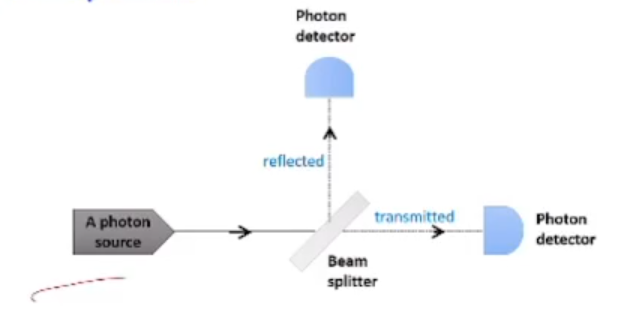
\includegraphics[scale=0.5]{1.png}
\end{center}
We send a series of individual photons along a path from the source towards the splitter. We expect two behaviors: the beam splitter transmits or reflects the photon. We observe the photon arriving at the detector on the right of the splitter half of the time, and arriving at the detector above half of the time.\\
So, we can model the splitter as flipping a fair coin, and choosing whether to transmit or reflect the photon based on the result of the coin-flip.\\\\
A beam splitter behaves like a fair coin: head (state 0) $\rightarrow$ transmitted, tail (state 1) $\rightarrow$ reflected. So both detectors will expect a photon with probability $\frac{1}{2}$
\subparagraph{Second experiment} We extend the experiment with two mirrors and another beam splitter.
\begin{center}
	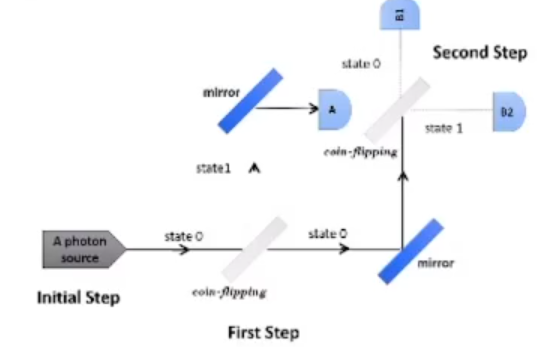
\includegraphics[scale=0.5]{2.png}
\end{center}
We have three detectors, and we observe a photon in A with probability $\frac{1}{2}$, and in B1 or B2 with probability both $\frac{1}{4}$.\\
Both experiments confirms our prediction.
\subparagraph{Third experiment} Let's remove the detector A.\begin{center}
	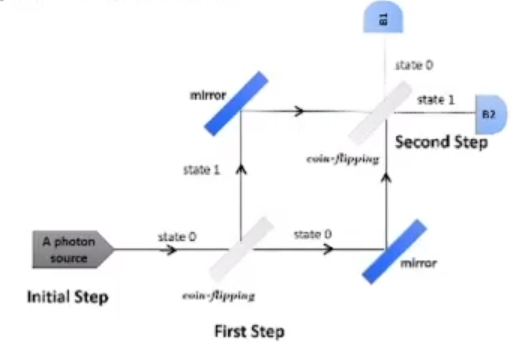
\includegraphics[scale=0.5]{3.png}
\end{center}
So we flip our photon, the "quantum coin", \textbf{without looking at the result of the first splitter}. What are the probabilities of observing the photon in B1 or B2? With the classical intuition, we expect $\frac{1}{2}$ probability in both and that's what would happen with a real "macroscopic" coin. So we predict to observe the photon in B1 and B2 evenly.\\
Let's see it in a mathematical way:
\begin{list}{}{}
	\item State 0: transmitted
	\item State 1: reflected
\end{list}
With a vector representation:
$$|0\rangle = \left(\begin{array}{c}
	1\\0
	\end{array}\right)\:\:\:\:\:\:\:\:|1\rangle = \left(\begin{array}{c}
	0\\1
	\end{array}\right)$$
With $|\:\:\rangle$ called \textbf{Dirac notation}, standard notation for states in quantum mechanics.\\
Uncertain states will be represented by linear combinations of $|0\rangle$ and $|1\rangle$
$$\alpha_0|0\rangle + \alpha_1|1\rangle = \alpha_0\left(\begin{array}{c}
1\\0
\end{array}\right) + \alpha_1\left(\begin{array}{c}
0\\1
\end{array}\right) = \left(\begin{array}{c}
\alpha_0\\\alpha_1
\end{array}\right)$$
With $\alpha_0,\alpha_1$ being the probabilities of finding the photon in state $|0\rangle$ or $|1\rangle$.\\
Since we should find the photon in exactly one path, we must have $\alpha_0+\alpha_1=1$\\\\
We model the splitter as randomly selecting whether the photon will be transmitted (state $|0\rangle$) or reflected (state $|1\rangle$)\\
After the initial step, we are in $|0\rangle$. We flip a coin (first splitter): the new probabilistic state is expected to be in both states with probability $\frac{1}{2}$
$$\frac{1}{2}|0\rangle + \frac{1}{2}|1\rangle = \left(\begin{array}{c}
\frac{1}{2}\\\frac{1}{2}
\end{array}\right)$$
The transition of a far coin can be represented by the matrix $$\left(\begin{array}{c c}
\frac{1}{2}&\frac{1}{2}\\\frac{1}{2}&\frac{1}{2}
\end{array}\right)$$
When the photon passes through the splitter, we multiply its state vector by this matrix, to derive the new state where the photon is expected to be in both states $|0\rangle$ and $|1\rangle$ with probability $\frac{1}{2}$
$$\left(\begin{array}{c c}
\frac{1}{2}&\frac{1}{2}\\\frac{1}{2}&\frac{1}{2}
\end{array}\right)\left(\begin{array}{c}
1\\0
\end{array}\right) = \left(\begin{array}{c}
\frac{1}{2}\\\frac{1}{2}
\end{array}\right) = \frac{1}{2}\left(\begin{array}{c}
1\\0
\end{array}\right) + \frac{1}{2}\left(\begin{array}{c}
0\\1
\end{array}\right)$$
Then we flip the coin again, and multiply the new state vector by the same matrix. The new probabilistic state will be the same:
$$\left(\begin{array}{c c}
\frac{1}{2}&\frac{1}{2}\\\frac{1}{2}&\frac{1}{2}
\end{array}\right)\left(\begin{array}{c}
\frac{1}{2}\\\frac{1}{2}
\end{array}\right) = \left(\begin{array}{c}
\frac{1}{2}\\\frac{1}{2}
\end{array}\right) = \frac{1}{2}\left(\begin{array}{c}
1\\0
\end{array}\right) + \frac{1}{2}\left(\begin{array}{c}
0\\1
\end{array}\right)$$
So our mathematical model confirms our expectations.\\\\
\textbf{The experimental results do not agree with our classical intuition!} We observe the photons \textbf{only in B1} and we \textbf{never observe any photon in B2}. This is the same problem which led to the development of quantum physics.
\paragraph{Quantum Physics} So let's use quantum physics to explain our experiments. "\textit{Quantum theory is probability theory with negative numbers}", but we can't have negative probabilities so we will use a new quantity called \textbf{amplitude}. To get around the fact that we cannot have negative probabilities and that all our probabilities must add up to 1, we use a mathematical trick: we square our amplitudes to calculate the probabilities.\\
According to the quantum mechanical description, the beam splitter causes the photon to go into a \textbf{superposition} of both states. Mathematically, we describe such superposition by taking a linear combination of the state vectors with $\alpha_0$ and $\alpha_1$ now being \textbf{complex numbers} $\in C$. If we measure the photon to see its state, we find it in state $|0\rangle$ with probability $|\alpha_0|^2$ and in state $|1\rangle$ with probability $|\alpha_1|^2$, and since a photon should be find in exactly one path, we need $|\alpha_0|^2+|\alpha_1|^2 = 1$\\\\
We start in state $|0\rangle=\left(\begin{array}{c}1\\0\end{array}\right)$. When it passes through the first splitter, we multiply its state vector with the matrix $$\left(\begin{array}{c c}
\frac{1}{\sqrt{2}}&\frac{1}{\sqrt{2}}\\\frac{1}{\sqrt{2}}&-\frac{1}{\sqrt{2}}
\end{array}\right)$$
After passing through the first splitter:
$$\left(\begin{array}{c c}
\frac{1}{\sqrt{2}}&\frac{1}{\sqrt{2}}\\\frac{1}{\sqrt{2}}&-\frac{1}{\sqrt{2}}
\end{array}\right)\left(\begin{array}{c}
1\\0
\end{array}\right) = \left(\begin{array}{c}
\frac{1}{\sqrt{2}}\\\frac{1}{\sqrt{2}}
\end{array}\right) = \frac{1}{\sqrt{2}}\left(\begin{array}{c}
1\\1
\end{array}\right)$$
Same as before, with $\frac{1}{\sqrt{2}}$ instead of $\frac{1}{2}$. The result correspond with the observed behavior: we measure the photon in state $|0\rangle$ with probability $\left(\frac{1}{\sqrt{2}}\right)^2=\frac{1}{2}$ and in state $|1\rangle$ with probability $\left(\frac{1}{\sqrt{2}}\right)^2=\frac{1}{2}$. The photon is in a \textbf{superposition} of states $|0\rangle$ and state $|1\rangle$, being in both states with amplitudes $\frac{1}{\sqrt{2}}$ and $\frac{1}{\sqrt{2}}$ respectively.\\
If we do not measure the state of the photon after passing through the first beam splitter, then its state remains $\frac{1}{\sqrt{2}}\left(\begin{array}{c}
1\\1
\end{array}\right)$. If the photon is allowed to pass through the second splitter before any measurement, the new state vector becomes
$$\left(\begin{array}{c c}
\frac{1}{\sqrt{2}}&\frac{1}{\sqrt{2}}\\\frac{1}{\sqrt{2}}&-\frac{1}{\sqrt{2}}
\end{array}\right)\cdot\frac{1}{\sqrt{2}}\left(\begin{array}{c}
1\\1
\end{array}\right) = \left(\begin{array}{c}
\frac{1}{2} + \frac{1}{2}\\\frac{1}{2}-\frac{1}{2}
\end{array}\right) = \left(\begin{array}{c}
1\\0
\end{array}\right)$$
The amplitude of the state $|0\rangle$ becomes 1, but the amplitude of the state $|1\rangle$ becomes 0 because \textbf{the amplitudes of finding the photon in state $|1\rangle$ cancel each other out}. We call this effect \textbf{interference}.\\
After being in both states at the same time with certain amplitudes, by passing through a second splitter the outcomes are interfered with each other: the interference can be destructive ($\frac{1}{2} - \frac{1}{2}$) or constructive ($\frac{1}{2} + \frac{1}{2}$).
\paragraph{What is Quantum Computing?} If we measure the photon, we find it coming out of state $|0\rangle$ with probability 1. Thus, after the second splitter the photon is entirely in state $|0\rangle$, which is what we observed.\\
In quantum "language": the second splitter has caused the two states (in superposition) to interfere, resulting in the cancellation of state $|1\rangle$.\\
The interference effects can be used to our advantage. We can combine operations such as the quantum coin toss to build more efficient algorithms. These algorithms can use interference effects to make the wrong answers cancel out quickly and give us high probabilities of measuring the right answer. This is the idea behind quantum computing.
\paragraph{Observations}\begin{list}{}{}
	\item This model works when the initial state is $|1\rangle$
	\item This model works also with complex numbers\\
	For instance we could use:
	\begin{list}{}{}
		\item Transition matrix: $\frac{1}{\sqrt{2}}\left(\begin{array}{c c}
		1&i\\i&1
		\end{array}\right)$
		\item Superposition of state $|0\rangle$ and $|1\rangle$: $\frac{1}{\sqrt{2}}\left(\begin{array}{c}
		i\\1
		\end{array}\right)$
		\item The model is consistent with the first and second experiment
		\begin{center}
			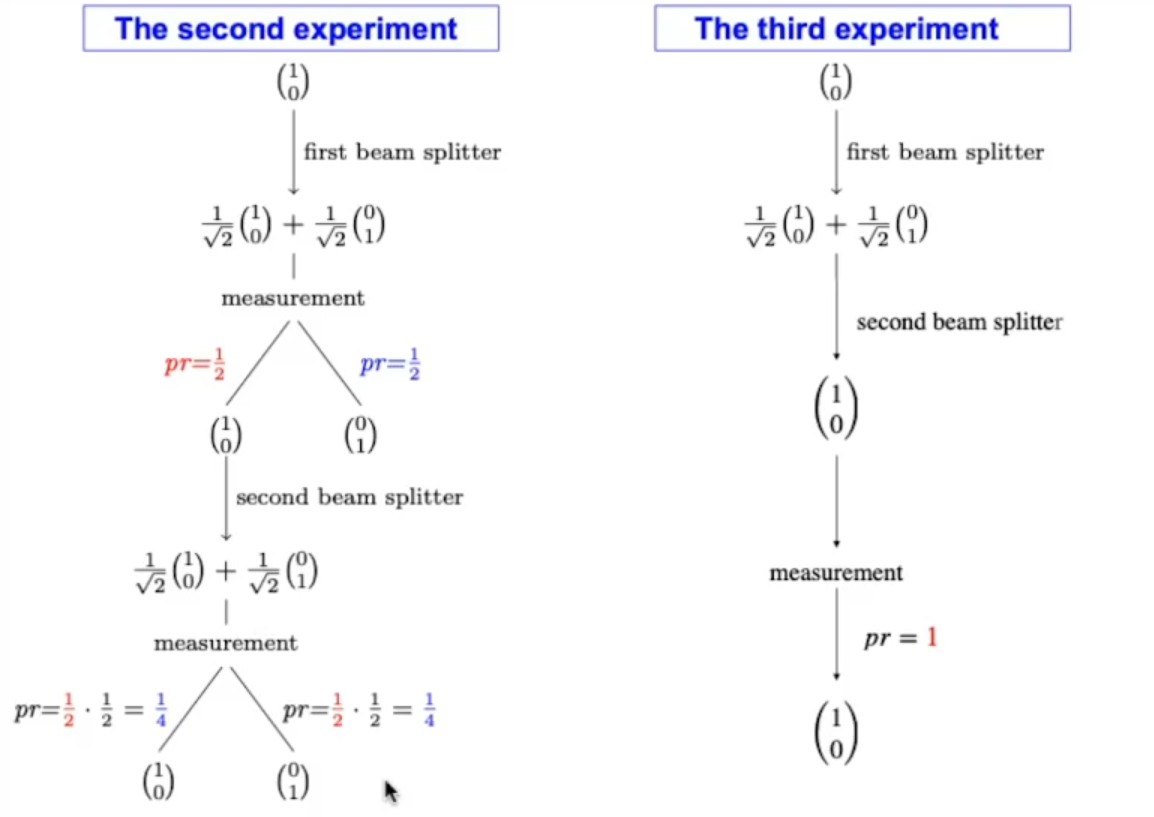
\includegraphics[scale=0.5]{4.png}
		\end{center}
	\end{list}
\end{list}
\paragraph{Phenomena of quantum mechanics that may intervene in the processing of information}
\begin{list}{}{}
	\item \textbf{Superposition} Property of a quantum system to be in different states at the same time.\\
	A quantum system can be in more than one state at the same time with non-zero amplitudes: we say that it's in a superposition of these states. When evolving from a superposition, the resulting transitions may affect each other constructively and destructively. This happens because of having opposite sign transition amplitudes
	\item \textbf{Decoherence} The attempt to observe or measure the state of the system causes its collapse towards a single state.\\
	The probability of a system to be observed in a specific state is the square value of its amplitude of a state. After the measurement, the system is no longer in a superposition: the information kept in the superposition is lost.\\
	The experimental manipulation of quantum systems is extremely difficult because every minimal disturbance can determine the decoherence.\\
	Qubits interact with their environments to some degree, even thought the physical substrate used to store them has been designed to keep the isolated.
	\item \textbf{No-Cloning} It's impossible to create an independent and identical copy of an arbitrary unknown quantum state
	\item \textbf{Entanglement} Possibility that two or more elements are in quantum states completely correlated with each other so that, even if transported at a great distance from each other, they maintain the correlation.
\end{list}
\subsection{Quantum Computer}
\paragraph{Bit and qubit} Conventional computers are made up of bits, while quantum computers are made up of quantum bits, or \textbf{qubits}.\\
A bit is the fundamental concept of classical computation: we can think of it in abstract terms as having a state which is either 0 or 1.\\
A qubit is the simplest of all quantum systems:
\begin{list}{}{}
	\item like a bit, it has a state
	\item two special states for qubits are the state $|0\rangle$ and $|1\rangle$, which correspond to states 0 and 1 of classical bits
	
$$|0\rangle = \left(\begin{array}{c}
	1\\0
	\end{array}\right)\:\:\:\:\:\:\:\:|1\rangle = \left(\begin{array}{c}
	0\\1
	\end{array}\right)$$
	These are called \textbf{computational basis states} and form an orthonormal basis for $C^2$
	\item The difference between bits and qubits is that a qubit can be in a state other than $|0\rangle$ and $|1\rangle$: it can be in a superposition of the two states simultaneously
	$$|\psi\rangle = \alpha|0\rangle+\beta|1\rangle$$
	\item The representation of information is binary, but each qubits contains double information with respect to a bit.
	\item We can examine a bit to determine if it's in state 0 or 1, but we cannot examine a qubit to determine it's quantum state (the values of $\alpha$ and $\beta$). We can only acquire much more restricted information about the quantum state.
	\item Measuring a qubit can only give classical results: either 0 with probability $|\alpha|^2$ or 1 with probability $|\beta|^2$\\
	Note that by measuring we lose information.
	\item A qubit $|\psi\rangle$ can be represented in a three-dimensional space as a point on the surface of a sphere of unitary radius known as \textbf{Bloch's sphere}.
\end{list}
\begin{center}
	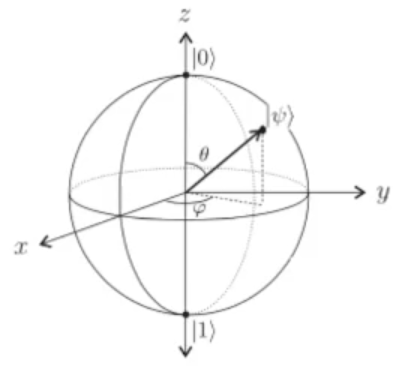
\includegraphics[scale=0.5]{5.png}
\end{center}
How much information in a qubit $|\psi\rangle = \alpha|0\rangle + \beta|1\rangle$? $\alpha$ is a complex number and we could store lots of bits in the binary expression of Re$(\alpha)$. This is there was some way of measuring the value of $\alpha$ exactly. But $\alpha,\beta$ are kind of hidden information. Measurement of a qubit will give only a single bit of information, 0 or 1, about the state of the qubit. There is no way to figure out $\alpha$ and $\beta$ if they start out unknown: after the measurement $\alpha$ and $\beta$ are gone.\\
Why does this collapse occurs? We don't know.\\
Only if infinitely many identically prepared qubits %TODO
\paragraph{Power of Quantum Computing} The system can be put in a combination of very large number of state: $n$ qubits in a superposition of $2^n$ states, so operating on $2^n$ bits at the same time.\\
Idea: find an algorithm that converges all $2^n$ states of the qubits to a state that's solution of the problem: exploiting constructive and destructive interferences, for example.
\paragraph{Quantum Algorithms} We start from a well known initial state (example: all qubits in $|0\rangle$). The system evolves in a quantum way: qubits are connected in elementary logic circuits and are manipulated by a simple set of rules (rotations of state vectors of the quantum state).\\
From a superposition of states to a superpositions of calculations (each with a certain probability of converging to a significant result) to a superposition of results. When the machine measures the final state, the superposition of results collapses on the result with the higher probability: with high probability being the solution of our problem.\\
This can be called \textbf{quantum parallelism}.\begin{list}{}{}
	\item Observing the system during these manipulations comes with a severe \textbf{penalty}: if we look to soon, the \textbf{computation will fail}. We are allowed to \textbf{view only the machine final state}.
	\item Interaction with the outside occurs through classic bit sequences: qubits collapses in that instant to a single state.
\end{list}
\paragraph{Why Quantum Computing?} The idea was born to efficiently simulate quantum-mechanical processes. But this model can help to solve problems of high computational complexity.\\
However:
\begin{list}{}{}
	\item Quantum computation doesn't violate the Church-Turing thesis, undecidable functions are still undecidable
	\item Widely believed that NP-Complete problems are still difficult problems, requiring exponential time
\end{list}
We are interested because for some problems a classical computers can take exponentially more time.
\paragraph{Shor's Factoring Algorithm} Factor numbers in polynomial time. This remains one of the (or \textit{the}) most important results in quantum computing. Meaning that \textbf{current public key cryptography can be attacked}. But remember that factorization is not NP-complete.
\paragraph{Grover's Quantum Search} The algorithm concerns search in an unstructured database with $N$ entries. If we are searching for a unique marked entry, classicaly it would take a maximum of $N$ queries and $\frac{N}{2}$ queries on average.\\
With this algorithm, enables the search to be completed with $O(\sqrt{N})$ queries. It's \textbf{optimal}: no search algorithm can do less than $\sqrt{N}$ operations.\\
In practice, this quadratic speed-up can be very impactful making a big difference. With $10^{20}$ entries, and a quantum processors capable of $10^8$ calls per second, we can find the entry in $10^{10}$ calls, so $10^2$ seconds ($\simeq 2$ minutes). In classical search we would need $10^{12}$ seconds ($\simeq 32000$ years).\\
In cryptography, it enables brute force attacks so we need longer keys.
\paragraph{Evolution of Quantum Technology}
%TODO image
\begin{center}
	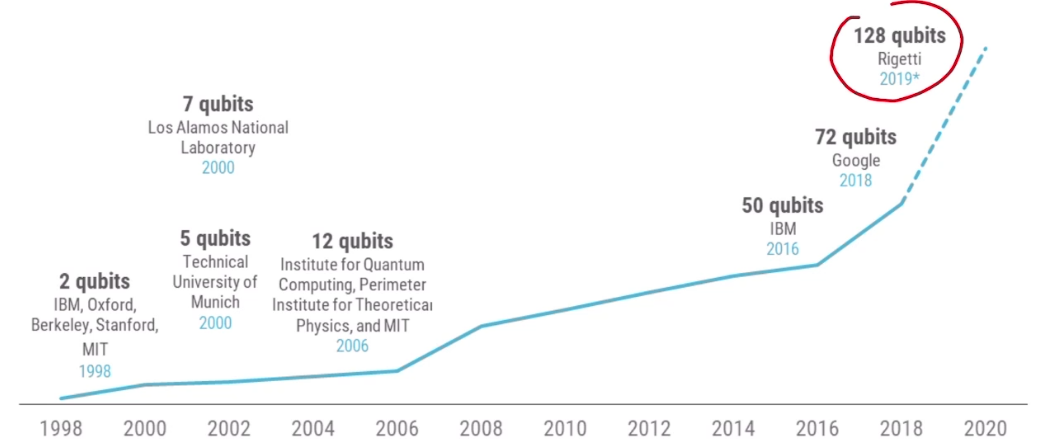
\includegraphics[scale=0.5]{6.png}
\end{center}
IBM claims that it will build a 1000-qubit machine by 2023 and 1M-qubits by 2030.
\paragraph{Quantum Supremacy} Is the goal of demonstrating that a programmable quantum device can solve a problem that \textbf{no classical computer can solve in any feasible amount of time} (irrespective of the usefulness of the problem).\\
Proving this requires:\begin{list}{}{}
	\item Building a powerful physical quantum machine
	\item Finding a problem that can be solved efficiently on a quantum computer with a superpolynomial speed-up over the best known or possible classical algorithm for that task.
\end{list}
Note that Shor's algorithm is unfeasible to be implemented with current technology, so it cannot be used to prove quantum supremacy.
\paragraph{Physical Realization of Quantum Computers}
A qubit can be realized as real quantum physical system. We can use:
\begin{list}{}{}
	\item Two different polarization of a photon
	\item Two possible alignments of nuclear spin in a uniform magnetic field
	\item Two state of an electron orbiting a single atom (ground or excited state, shining light on the electron makes it change states and even stay halfway between states)
\end{list}
The theory is independent of the physical realization of the system.
\begin{center}
	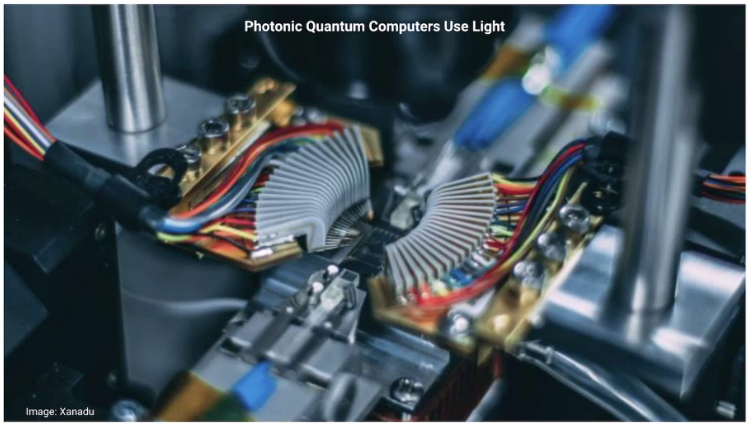
\includegraphics[scale=0.5]{7.png}
	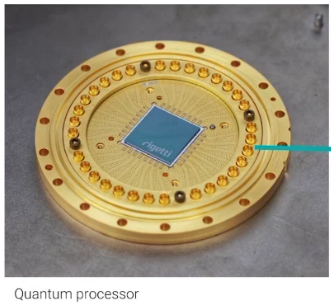
\includegraphics[scale=0.7]{8.png}
\end{center}
\paragraph{Challenges} It will be quite an engineering challenge to control a quantum computer and to make sure that its state will not be affected by various sources of error.\\
Quantum operations (rotations) are never perfect: an intended rotation of 90 degrees might end up being of 90.1 or 89.9 degrees and this errors add up quickly.\\
It's very difficult to avoid interaction with the external environments, so need fault-tollerant protocols and quantum-errors correcting algorithms, meaning additional qubits.\\
Circuit dimensions are also very large. Shor's algorithm require $O(n^2\log n\log\log n)$ gates for a $n$ bit number.
\section{Circuit Model of Computation}
\begin{center}
	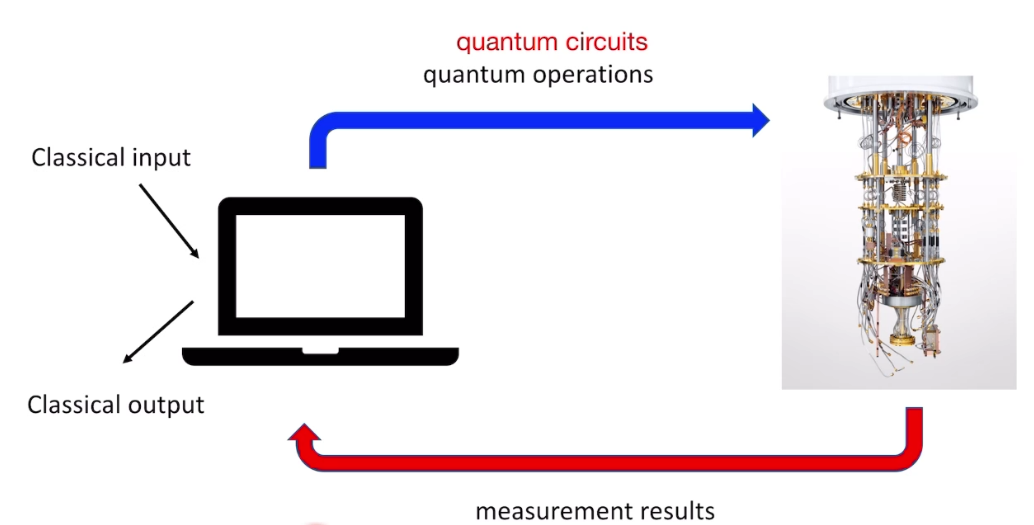
\includegraphics[scale=0.5]{9.png}
\end{center}
The \textbf{interaction is classical}.
\paragraph{Circuits} Networks (graphs) of wires (arcs) that carry bit values to gates that perform elementary operations (nodes) on the bits (input nodes).\\
$C_n$ circuit with $n$ input variables. We consider acyclic circuits. The gates come from some finite library of gates.\\
Circuits are a \textbf{non-uniform model of computation}: with $n$ inputs we can solve only instances of length $n$. Inputs of different lengths are processed by different circuits, in contrast with uniform models (such as Turing machines) where the same computational device is used for all possible input lengths. A different "program" for each input size.\\\\Non-uniform because computation on input size $n$ can be absolutely different from computations on some input size $m$. For example, \textbf{non-uniform circuit families of small size may compute undecidable functions}. Size being the number of operations in the circuit.\begin{list}{}{}
	\item Let $L\subseteq \{0,1\}^*$ be an undecidable language
	\item Let $U = \{1^n\:|\:$the binary expansion of $n$ is in $L\}$\\
	For example $1^5 = 11111_1\in U$ if $5_{10}=101_2 \in L$
	\item $U$ is also undecidable, but we can build a non-uniform family of circuits that computes $U$: $\forall\:n$ we build two circuits with $n$ inputs\begin{list}{}{}
		\item $C_n^0$ %TODO
		\item $C_n^1$ %TODO
	\end{list}
	What's missing is the effective and efficient constructability of the circuits. Since $U$ is undecidable we are not able to say if the $n$-th circuit of the family is $C_n^0$ or $C_n^1$.
\end{list}
\paragraph{Uniform Families} So we often impose a \textbf{uniformity condition}: the family is uniform if each $C_n$ can be constructed by an appropriately resource-bounded Turing machine. We assume that the circuits can be generated by a Turing machine or equivalent model that on input $n$ produces a description of $C_n$ in time polynomial in $n$ and in the number of gates in $C_n$.
\paragraph{Complexity of the Circuits} One natural measure is the \textbf{overall number of gates}, the number of operations (can be put in relation with sequential time).\\
Another is the \textbf{depth of the circuit}, the length of the longest path between input and output with each gate counting as one, can be put in relation with parallel time.\\
A third measure is the \textbf{number of input variables}, sometimes called width or space of the circuit.
\paragraph{Reversible Computation} Quantum computation are always reversible. A computation is reversible if it always possible to uniquely recover the input given the output. Otherwise, it's called irreversible.\\
Many classical logic gates are irreversible, but the NOT gate is reversible.\\
Reversibility is connected to information loss: an irreversible operation produces loss of information. With reversible computation no information is ever erased.\\
Laws of physics %TODO
\paragraph{Reversible Circuits} Realize bijection. We have digital circuits with same number of input and outputs. Any classical irreversible circuit can be transformed in a equivalent reversible one (computes same one), by adding new inputs and new outputs and replacing irreversible operations with reversible ones. The extra inputs represent information that we must keep in order to maintain the reversability.\\
With an irreversible classical circuit of depth $T$ and space $S$, the reversible version uses $O(S+ST)$ space and $T$ depth.
\subparagraph{Reversible AND} Also known as Toffoli gate.
\begin{center}
	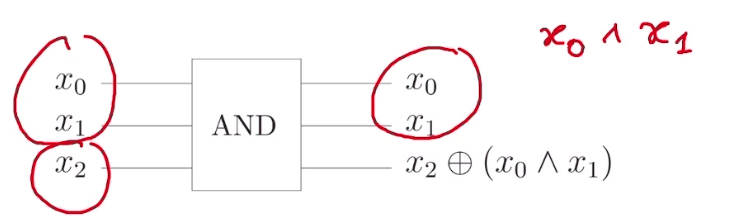
\includegraphics[scale=0.5]{10.png}
\end{center}
\paragraph{Universality} A set of gates is universal for classical computation if, for any positive integer $n,m$ and any function $f : \{0,1\}^n\rightarrow \{0,1\}^m$, a circuit can be constructed for computing $f$ using only gates from that set.\\
Well-known sets are \{AND, OR, NOT\}\ldots \\ %TODO 
NAND and NOR gates have the \textbf{functional completeness} assuming unlimited unlimited fanout (a gate can be connected to unlimitedely many nodes).\\\\
\textbf{Toffoli gate} is universal for classical reversible computation. We need to add \textbf{ancillary} (extra) bits that can be initialized to 0 or 1 as required.
\section{Complex Numbers}
A field that can be represented in a 2D space.
$$z = a + ib$$ with $a,b \in R$ and $i^2 = -1$, that can be represented in a plot with $Re(z) = a$ on $x$ axis and $Im(z) = b$ on $y$ axis (\textbf{cartesian form}).\\
Can be expressed also as $$z = \rho(\cos\theta + i \sin\theta) = \rho \cdot e^{i\theta}$$ with $\rho$ being the distance from the origin and $\theta$ the angle (\textbf{polar form}). $\rho$ is called modulo and $e^{i\theta}$ is called phase (sometimes referring with that term to just $\theta$)
$$|z|^2 = z\cdot z^* = a^2 + b^2 = \rho^2 = |z^*|$$
$$z^* = \overline{z} = a-ib = \rho(\cos\theta - i\sin\theta) = \rho\cdot e^{-i\theta}$$
with $\overline{z}$ called complex conjugate of $z$.
\paragraph{Euler Identity} Let's prove the polar form. $e^z$ is a function from $C$ to $C$
$$e^z = \sum_{k=0}^\infty = \frac{z^k}{k!}$$
With $z\in C$, let's see with $z = ix$ and $x\in R$. We want to prove that
$$e^{ix} = \cos x + i\sin x$$
\pagebreak
$$e^{ix} = \sum_{k=0}^\infty \frac{(ix)^k}{k!} = 1 + ix + \frac{i^2x^2}{2} + \frac{i^3x^3}{3!} + \ldots=$$
Let's take the even powers, we have $i^2 = -1, i^4 = +1,\ldots$, and with the odd powers we can take out $i$ from the $\sum$
$$= \sum_{k=0}^\infty \frac{(-1)^{k}x^{2k}}{(2k)!} + i\sum_{k=0}^\infty \frac{(-1)^k x^{2k+1}}{(2k+1)!} =$$
These are the power series expansions of $\cos$ and $\sin$
$$e^{ix}=\cos x + i \sin x$$
This results in the Euler identity which puts together all the principle of math. The imaginary unit an two irrational number together with $1$ and $0$.
$$e^{i\pi} + 1 = 0 \Leftrightarrow e^{i\pi} = -1$$
\paragraph{Roots of Unity} Useful when we want to solve $z^n - 1 = 0$. We know that every polynomial has exactly $n$ roots in $C$\\
Primitive $n$th root of 1
$$\omega_n = e^{\frac{2\pi i}{n}} = \cos \frac{2\pi}{n} + i \sin\frac{2\pi}{n}$$
So for example $\omega_3 = \cos\frac{2}{3}\pi + i\sin\frac{2}{3}\pi = \frac{1}{2}+i\frac{\sqrt{3}}{2}$ for $z^3 - 1 = 0$\\
So they are counterclockwise on the unitary circle and also unitary roots are cyclic
$$w_n^k = (\cos \frac{2\pi}{n} + i \sin\frac{2\pi}{n})^k = \cos\frac{2\pi}{n}k + i \sin\frac{2\pi}{n}k = \left(e^{\frac{2\pi i}{n}}\right)^k$$
\begin{list}{}{}
	\item $\omega_n^0 = 1$
	\item $\omega_n^{n+k} = \omega_n^n \cdot \omega_n^k = \omega_n^k$
	\item $\omega_n^{n-k} = \omega_n^n \cdot \omega_n^{-k} = \omega_n^{-k}$
\end{list}
Multiplication and division are easier in the polar form
$$z_1\cdot z_2 = \rho_1\cdot\rho_2(\cos(\theta_1+\theta_2) + i\sin(\theta_1+\theta_2))$$
$$\frac{z_1}{z_2} = \frac{\rho_1}{\rho_2}(\cos(\theta_1-\theta_2) + i\sin(\theta_1-\theta_2))$$
$$z^n = \rho^n\cdot e^{in\theta}$$
\subsection{Hilbert Spaces} For Quantum Computing only finite dimensional Hilbert spaces meaning complex vector spaces with an inner product.
\paragraph{Definition} A quantum state space of a system is a vector space (complex) with inner product.\\
For example, photon polarization: we have a basis and it's a 2-dimensional space. Base states are $|\updownarrow\rangle$ and $|\leftrightarrow\rangle$. We use half-spin patches, $|\uparrow\rangle$ spin up and $|\downarrow\rangle$ spin down.\\
If we consider a 4-dimensional state space, we have $4$ vectors in the base:$|0\rangle$, $|1\rangle$, $|2\rangle$, $|3\rangle$ denoted with $$|v\rangle=\left(\begin{array}{c}
v_0\\v_1\\v_2\\v_3
\end{array}\right)$$ using the ket notation.
\paragraph{Definition} A quantum state is a vector of unitary length in a quantum state space.\\
So $\| |v\rangle\| = 1$, $\|v\|=\sqrt{(v,v)}$ with the inner product defined as
$$(v,w)=\sum_{i=1}^{d-1}v_i^*\cdot w_i$$
We can use the bra $$\langle v| = (v_0^*,\ldots,v_{d-1}^*)$$
$$\langle v\:|\:w\rangle = (v,w)\in C$$
or the ket-bra $$|v\rangle\langle w| = (v_iw_j^*)_{i,j}$$ giving a rank-one matrix.
\paragraph{} For a system of 1 qubit we have as basis $$|0\rangle = \left(\begin{array}{c}
1\\0
\end{array}\right), |1\rangle=\left(\begin{array}{c}
0\\1
\end{array}\right)$$ but we can also denote this as $|\uparrow\rangle$ and $|\downarrow\rangle$ and denote as $$|\rightarrow\rangle = \frac{|\uparrow\rangle + |\downarrow\rangle}{\sqrt{2}}$$
$$|\leftarrow\rangle = \frac{|\uparrow\rangle - |\downarrow\rangle}{\sqrt{2}}$$
as spin-right and spin-left.\\
We can define spin-in ("in the board")
$$|\otimes\rangle = \frac{|\uparrow\rangle + i|\downarrow\rangle}{\sqrt{2}}$$
and spin-out ("out of the board")
$$|\bullet\rangle = \frac{|\uparrow\rangle - i|\downarrow\rangle}{\sqrt{2}}$$
Multiplying a quantum state bu a global phase ($e^{i\theta}$) we do not change the nature of the quantum state. A global phase is a quantity that multiply all the components of the basis vector.
$$|\rightarrow\rangle = \frac{|\uparrow\rangle + |\downarrow\rangle}{\sqrt{2}} \neq \frac{|\uparrow\rangle + i|\downarrow\rangle}{\sqrt{2}} = |
\otimes\rangle$$
In the above case, $i$ is a relative phase.
\paragraph{Bloch Sphere} %TODO
\begin{center}
	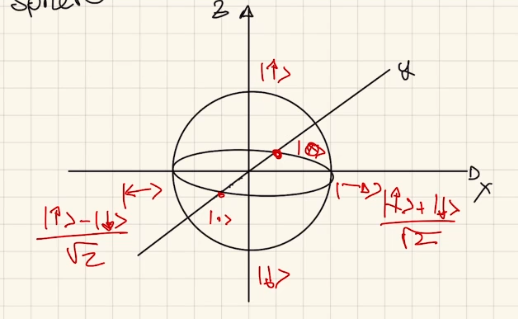
\includegraphics[scale=0.5]{11.png}
\end{center}
\paragraph{Pauli Matrices} $$X = \sigma_x = \left(\begin{array}{c c}
0&1\\1&0
\end{array}\right)$$
$$\sigma_x|0\rangle = \left(\begin{array}{c c}
0&1\\1&0
\end{array}\right)\cdot\left(\begin{array}{c}
1\\0
\end{array}\right) = \left(\begin{array}{c}
0\\1
\end{array}\right) =|1\rangle$$
It reflects the points along the $x$ axis. The same goes for $\sigma_x|1\rangle = |0\rangle$.\\
So for the points on the $x$ axis stay almost the same.
$$|\rightarrow\rangle = \frac{|0\rangle + |1\rangle}{\sqrt{2}} = \frac{1}{\sqrt{2}}\left(\begin{array}{c}
1\\1
\end{array}\right)$$
$$\sigma_x|\rightarrow\rangle = \frac{1}{\sqrt{2}}\left(\begin{array}{c}
1\\1
\end{array}\right)$$
The $y$ axis Pauli matrix is $$Y = \sigma_y = \left(\begin{array}{c c}
0&-i\\i&0
\end{array}\right) = -i|0\rangle\langle1| + i |1\rangle\langle0|$$
and the last is $$Z = \sigma_z = \left(\begin{array}{c c}
1&0\\0&-1
\end{array}\right) = |0\rangle\langle0| - |1\rangle\langle1|$$
\subparagraph{Theorem} The three Pauli matrices anticommutes
$$\sigma_i\sigma_j = -\sigma_j\sigma_i$$
for $i,j\in\{x,y,z\}$ and $i\neq j$\\
Also $\sigma_i^2 = I$
\paragraph{Hadamard Matrix} Another important matrix, used for building entangled states.
$$H=\frac{1}{\sqrt{2}}\left(\begin{array}{c c}
1&1\\1&-1
\end{array}\right)$$
It allow to move from the canonical basis to the right-left basis (also known as +- basis).
$$H|0\rangle = \frac{1}{\sqrt{2}}\left(\begin{array}{c}
1\\1
\end{array}\right) = |\rightarrow\rangle = |+\rangle$$
$$H|1\rangle = \frac{1}{\sqrt{2}}\left(\begin{array}{c}
1\\-1
\end{array}\right) = |\leftarrow\rangle = |-\rangle$$
Also $H^2 = I$, $H^{-1} = H$ so $|0\rangle\mapsto_H |+\rangle$ and $|+\rangle\mapsto_H |0\rangle$ same with $|1\rangle$ and $|-\rangle$, "back and forth".\\
$$H|\otimes\rangle = \frac{1}{\sqrt{2}}\left(\begin{array}{c c}
1&1\\1&-1
\end{array}\right)\left(\begin{array}{c}
\frac{1}{\sqrt{2}}\\\frac{1}{\sqrt{2}}i
\end{array}\right) = |\bullet\rangle$$
\paragraph{Other common single qubit gates} Already mentioned $X,Y,Z,H$\begin{list}{}{}
	\item $I = \left(\begin{array}{c c}
	1&0\\0&1
	\end{array}\right)$
	\item $S = \left(\begin{array}{c c}
	1&0\\0&e^{i\frac{\pi}{2}}
	\end{array}\right)$
	\item $T = \left(\begin{array}{c c}
	1&0\\0&e^{i\frac{\pi}{4}}
	\end{array}\right)$
\end{list}
\end{document}